\clearpage

% Use different numbering in appendix to make it clear that a
% section/table/algorithm is not in the main text
\renewcommand\thefigure{\thesection\arabic{figure}}
\renewcommand\thetable{\thesection\arabic{table}}
\renewcommand{\theequation}{\thesection\arabic{equation}}

% modified title header from main page, code extracted from NeurIPS template
\makeatletter
\vbox{%
  \hsize\textwidth
  \linewidth\hsize
  \vskip 0.1in
  \@toptitlebar
  \centering
  {\LARGE\bf \@title (Supplementary Material)\par}
  \@bottomtitlebar
  \vskip 0.3in \@minus 0.1in
}
\makeatother

% APPENDIX TOC
\startcontents[sections]
\printcontents[sections]{l}{1}{\setcounter{tocdepth}{2}}
\vspace{2em}

\section{Example: Laplacian for a Shallow Network}


\section{Example: Laplacian for a Shallow Network}

Here, we compute the Laplacian for a less general, yet simpler, example: A shallow neural network.

\begin{comment}
  For the one-dimensional shallow case we have
  \[ u_\theta(x) = \sum_{i=1}^m a_i\sigma(b_i x + c_i) + d. \]
  Then
  \[ u_\theta'(x) = \sum_{i=1}^m a_ib_i\sigma'(b_i x + c_i) \]
  and
  \[ u_\theta''(x) = \sum_{i=1}^m a_ib_i^2\sigma''(b_i x + c_i). \]
  The parameter derivative of the Laplacian (i.e., second-order derivative)
  \begin{align*}
    \partial_{a_i}u_\theta''(x) & = b_i^2\sigma''(b_i x + c_i) \\
    \partial_{b_i}u_\theta''(x) & = 2a_ib_i\sigma''(b_i x + c_i) + a_i b_i^2x\sigma^{(3)}(b_i x + c_i) \\
    \partial_{c_i}u_\theta''(x) & = a_i b_i^2\sigma^{(3)}(b_i x + c_i) \\
    \partial_{d}u_\theta''(x) & = 0.
  \end{align*}
  The parameter derivative of the Laplacian (i.e., second-order derivative)
  \begin{align*}
    \partial_{a_i}u_\theta''(x) & = b_i^2\sigma''(b_i x + c_i) \\
    \partial_{b_i}u_\theta''(x) & = 2a_ib_i\sigma''(b_i x + c_i) + a_i b_i^2x\sigma^{(3)}(b_i x + c_i) \\
    \partial_{c_i}u_\theta''(x) & = a_i b_i^2\sigma^{(3)}(b_i x + c_i) \\
    \partial_{d}u_\theta''(x) & = 0.
  \end{align*}
\end{comment}

First, we do the Hessian calculation as explicitly as possible. For this, we consider the easy case of a shallow network with one-dimensional output
\[ u_\theta(x) = \sum_{i=1}^m a_i\sigma(b_i^\top x + c_i) + d. \]
Then
\[ \nabla_x u_\theta(x) = \sum_{i=1}^m a_ib_i\sigma'(b_i x + c_i) \]
or
\[ \partial_{x_j} u_\theta(x) = \sum_{i=1}^m a_i(b_i)_j\sigma'(b_i x + c_i). \]
Consequently, we compute
\[ \partial_{x_k}\partial_{x_j} u_\theta(x) = \sum_{i=1}^m a_i(b_i)_j(b_i)_k\sigma'(b_i x + c_i) \]
which yields the Hessian
\[ \nabla^2_x u_\theta(x) = \sum_{i=1}^m a_i\sigma''(b_i x + c_i) \cdot b_ib_i^\top = \sum_{i=1}^m a_i\sigma''(b_i x + c_i) \cdot  b_i\otimes b_i \]
and the Laplacian is given by
\[ \Delta_x u_\theta(x) = \sum_{i=1}^m a_i\sigma''(b_i x + c_i) \operatorname{tr}(b_ib_i^\top) = \sum_{i=1}^m a_i\sigma''(b_i x + c_i)  \operatorname{tr}(b_i\otimes b_i). \]
The parameter derivatives of the Hessian are given
\begin{align*}
  \partial_{a_i}\nabla_x^2 u_\theta(x) & = \sigma''(b_i x + c_i) b_ib_i^\top \\
  \nabla_{b_i}\nabla_x^2 u_\theta(x) & = a_i\sigma''(b_i x + c_i) (b_i\otimes I+I\otimes b_i) + a_i \sigma^{(3)}(b_i x + c_i) \cdot  (I\otimes x^\top)(b_i\otimes b_i) \quad ?? \\
  % + a_i x\sigma^{(3)}(b_i x + c_i) \cdot b_ib_i^\top \\
     \partial_{c_i}\nabla_x^2 u_\theta(x) & = a_i b_i^2\sigma^{(3)}(b_i x + c_i) \\
     \partial_{d}\nabla_x^2 u_\theta(x) & = 0.
\end{align*}
The parameter derivatives of the Laplacian are given
\begin{align*}
     \partial_{a_i}\Delta_x u_\theta(x) & = \sigma''(b_i x + c_i) \operatorname{tr}(b_ib_i^\top) \\
     \nabla_{b_i}\Delta_x u_\theta(x) & = 2a_i\sigma''(b_i x + c_i) + a_i \sigma^{(3)}(b_i x + c_i) \operatorname{tr}(b_ib_i^\top) \cdot x \\
     \partial_{c_i}\Delta_x u_\theta(x) & = a_i \sigma^{(3)}(b_i x + c_i)\operatorname{tr}(b_ib_i^\top) \\
     \partial_{d}\Delta_x u_\theta(x) & = 0.
\end{align*}


\paragraph{Writing as linear algebra}

Consider a shallow network
\[ u_\theta(x) = W_2\sigma(W_1 x), \]
where $x\in\mathbb R^d$, $W_1\in\mathbb R^{m\times d}, W_2\in\mathbb R^{1\times m}$.

\paragraph{Task: }
Understand the structure, in particular the computational graph of $f_\theta = \Delta u_\theta$.

\paragraph{One dimensional case: }
Assume first that $d=1$.
Then
\[ D_x u_\theta(x) = W_2 \operatorname{diag}(\sigma'(W_1 x)) W_1 \]
and
\[ D^2_x u_\theta(x) = W_2%(W_1^\top\otimes W_2)
  \operatorname{diag}(\operatorname{diag}(\sigma''(W_1 x)) W_1)W_1. % = W_2 \operatorname{diag}\sigma''(W_1 x) W_1^2 = W_2\odot W_1^2 \sigma''(W_1x),
\]
In another form
\[D^2 u_\theta(x) = W_2 \operatorname{diag}(\operatorname{diag}\sigma''(W_1 x) W_1) W_1 = W_2 \operatorname{diag}\sigma''(W_1 x) W_1^2 = W_2\odot W_1^2 \sigma''(W_1x),
\]
where $(W_2\odot W_1^2)_k = (W_2)_k \cdot (W_1)_k^2$.
% where $(W_2\odot W_1^2)_k = (W_2)_k \cdot (W_1)_k^2$.
% The Laplacian is then given as
% \[ f_\theta(x) = \Delta u_\theta(x) = \operatorname{tr}(D_x^2u_\theta(x)) =\operatorname{tr}(W_2 \operatorname{diag}(\operatorname{diag}(\sigma''(W_1 x)) W_1) W_1).  \]
% Differentiation with respect to $W_2$ yields
% \[ \frac{\partial f_\theta(x)}{\partial W_2} = \frac{\partial \Delta u_\theta(x)}{ \partial W_2} =  \]

One can also rewrite the diagonalization operator via a Hadamard product as $\operatorname{diag}(x) = (x\mathds{1}^\top)\odot I$, where $\mathds{1}$ denotes the all one vector, $I$ the identity and $\odot$ the Hadamard (i.e., entrywise) product of two matrices.
Not sure whether this helps though...

\paragraph{Multi-dimensional case}

%%% Local Variables:
%%% mode: latex
%%% TeX-master: "../main"
%%% End:


\section{Inverting the Sum of Two Kronecker Matrices}\label{sec:inverse_kronecker_sum}
PINNs use two losses: a boundary and an interior loss.
When designing a Kronecker-factored curvature approximation, we have two choices:
\begin{enumerate}
\item We can approximate each loss individually with a Kronecker product, i.e.
  \begin{align*}
    \mK \coloneqq \mA_1 \otimes \mA_2 + \mB_1 \otimes \mB_2
  \end{align*}
  where $\mA_{1,2}, \mB_{1,2}$ are invertible and positive definite.

\item We can further approximate the above through a single Kronecker product, e.g.\,by summing,
  \begin{align*}
    \mK' \coloneqq (\mA_1 + \mB_1) \otimes (\mA_2 + \mB_2) \approx \mK\,.
  \end{align*}
\end{enumerate}
Eventually, we want to use their inverses.
For $\mK'$, this is straightforward to do.
For $\mK$, we need to invert the sum of two Kronecker products, which is more challenging.
We can proceed as follows to invert $\mK$:
\begin{enumerate}
\item Simultaneously diagonalize $(\mA_i, \mB_i)$ by solving the generalized eigenvalue problem
  \begin{align*}
    \mA_i \mV_i = \mB \mV_i \mLambda_i
  \end{align*}
  where $\mV_i$'s columns are the (generalized) eigenvectors and $\mLambda_i$ is a diagonal matrix containing the (generalized) eigenvalues.

\item Consider the expression
  \begin{align*}
    &\left(
      \mA_1 \otimes \mA_2
      +
      \mB_1 \otimes \mB_2
      \right)
      \left(
      \mV_1 \otimes \mV_2
      \right)
    \\
    &=
      \mB_1 \mV_1 \mLambda_1 \otimes \mB_2 \mV_2 \mLambda_2
      +
      \left( \mB_1 \otimes \mB_2 \right)
      \left( \mV_1 \otimes \mV_2 \right)
    \\
    &=
      \left( \mB_1 \otimes \mB_2 \right)
      \left( \mV_1 \otimes \mV_2 \right)
      \left(
      \mLambda_1 \otimes \mLambda_2 + \mI \otimes \mI
      \right)\,.
  \end{align*}
  Rearrange into
  \begin{align*}
    \left(
    \mA_1 \otimes \mA_2
    +
    \mB_1 \otimes \mB_2
    \right)
    =
    \left( \mB_1 \otimes \mB_2 \right)
    \left( \mV_1 \otimes \mV_2 \right)
    \left(
    \mLambda_1 \otimes \mLambda_2 + \mI \otimes \mI
    \right)
    \left( \mV_1^{-1} \otimes \mV_2^{-1} \right)
    \,.
  \end{align*}

  \item Take the inverse to obtain
    \begin{align*}
      \mK^{-1}
      =
      \left( \mV_1 \otimes \mV_2 \right)
      \left(
      \mLambda_1 \otimes \mLambda_2 + \mI \otimes \mI
      \right)^{-1}
      \left( \mV_1^{-1}\mB_1^{-1} \otimes \mV_2^{-1}\mB_2^{-1} \right)
      \,.
    \end{align*}
    Notice that $\mLambda_1 \otimes \mLambda_2 + \mI \otimes \mI$ is diagonal, and therefore easy to invert.
\end{enumerate}

%%% Local Variables:
%%% mode: latex
%%% TeX-master: "../main"
%%% End:




\section{Taylor-Mode Automatic Differentiation \& Forward Laplacian}
PINN losses involve differential operators of the neural network, for instance the Laplacian.
Recently, \citet{li2023forward} proposed a new computational framework called \emph{forward Laplacian} to evaluate the Laplacian and the neural network's prediction in one forward traversal.
To establish a Kronecker-factorized approximation of the Gramian, which consists of the Laplacian's gradient, we need to know how a weight matrix enters its computation.
Here, we describe how the weight matrix of a linear layer inside a feed-forward net enters the Laplacian's computation when using the forward Laplacian framework.
We start by connecting the forward Laplacian framework to Taylor-mode automatic differentiation \citep{griewank2008evaluating,bettencourt2019taylor}, both to make the presentation self-contained and to explicitly point out this connection which we believe has not been done previously.

\subsection{Taylor-Mode Automatic Differentiation}\label{sec:taylor-mode-tutorial}
The idea of Taylor-mode is to forward-propagate Taylor coefficients, i.e.\,directional derivatives, through the computation graph. We provide a brief summary based on its description in \cite{bettencourt2019taylor}.

\paragraph{Taylor series and directional derivatives} Consider a function $f: \sR^d \to \sR$ and its $K$-th order Taylor expansion at a point $\vx \in \sR^d$ along a direction $\alpha \vv \in \sR^d$ with $\alpha \in \sR$,
\begin{align*}
  \hat{f}(\alpha) =
  f(\vx + \alpha \vv)
  &=
    f(\vx)
    +
    \alpha
    \left(
    \frac{\partial f(\vx)}{\partial \vx}
    \right)^{\top} \vv
    +
    \frac{\alpha^2}{2!}
    \vv^\top
    \left(
    \frac{\partial^2 f(\vx)}{\partial \vx^2}
    \right) \vv
  \\
  &\phantom{=}+
    \frac{\alpha^3}{3!}
    \sum_{i_1, i_2 i_3}
    \left(
    \frac{\partial^3 f(\vx)}{\partial\vx^3}
    \right)_{i_1, i_2, i_3} \evv_{i_1} \evv_{i_2} \evv_{i_3}
  \\
  &\phantom{=}+
    \ldots
  \\
  &\phantom{=}+
    \frac{\alpha^K}{K!}
    \sum_{i_1, \dots, i_K}
    \left(
    \frac{\partial^K f(\vx)}{\partial\vx^K}
    \right)_{i_1, \dots, i_K} \evv_{i_1} \cdots \evv_{i_K}\,.
\end{align*}
We can unify this expression by introducing the $K$-th order directional derivative of $f$ at $\vx$ along $\vv$,
\begin{align*}
  \partial^K f(\vx)
  \underbrace{\left[ \vv, \ldots, \vv \right]}_{K\,\text{times}}
  \coloneqq
  \sum_{i_1, \dots, i_K}
  \left(
  \frac{\partial^K f(\vx)}{\partial\vx^K}
  \right)_{i_1, \dots, i_K} \evv_{i_1} \dots \evv_{i_K}\,.
\end{align*}
This simplifies the uni-directional Taylor expansion to
\begin{align*}
  \hat{f}(\alpha) = f(\vx + \alpha\vv)
  &=
    f(\vx)
    +
    \alpha
    \partial f(\vx)[\vv]
    +
    \frac{\alpha^2}{2!}
    \partial^2 f(\vx)[\vv, \vv]
    +
    \frac{\alpha^3}{3!}
    \partial^3 f(\vx)[\vv, \vv, \vv]
  \\
  &\phantom{=}+
    \ldots
    +
    \frac{\alpha^K}{K!}
    \partial^K f(\vx)[\vv, \ldots, \vv]
  \\
  &\eqqcolon
    \sum_{k=1}^K
    \frac{\alpha^k}{k!}
    \partial^k f(\vx)\left[\otimes^k \vv  \right]
    \eqqcolon
    \sum_{k=1}^K
    w^f_k \alpha^k
\end{align*}
where we have used the notation $\otimes^k \vv$ to indicate $k$ copies of $\vv$, and introduced the $k$-th order Taylor coefficient $w^f_k \in \sR$ of $f$.
This generalizes to vector-valued functions:
If $f$'s output was vector-valued, say $f(\vx) \in \sR^c$, we would have Taylor-expanded each component individually and grouped coefficients of same order into vectors $\vw_k^f \in \sR^c$ such that $[\vw_k^f]_i$ is the $k$-th order Taylor coefficient of the $i$th component of $f$.

\paragraph{A note on generality:} In this introduction to Taylor-mode, we limit the discussion to the computation of higher-order derivatives along a single direction $\vv$, i.e.\,$\partial^Kf(\vx)[\vv, \dots, \vv]$.
This is limited though, e.g.\,if we set $K=2$ then we can compute $\partial^2 f(\vx)[\vv, \vv] = \vv^{\top} (\nicefrac{\partial^2 f(\vx)}{\partial\vx^2}) \vv$.
We can set $\vv = \ve_i$ to the $i$-th standard basis vector to compute the $i$-th diagonal element of the Hessian.
But we cannot evaluate off-diagonal elements, as this would require multi-directional derivatives, like $\partial^2 f(\vx) [\ve_i, \ve_{j\neq i}]$.
A more general description of Taylor-mode for multi-directional Taylor series along $M$ directions, $\hat{f}(\alpha_1, \dots, \alpha_M) = f(\vx + \alpha_1 \vv_1 + \dots + \alpha_M \vv_M)$, which require more general directional derivatives $\partial^K f(\vx) [\vv_1, \dots, \vv_K]$ (each vector can be different) are discussed in \cite{johnson2021taylor-made}.
We will use this formulation later to generalize the forward Laplacian scheme to more general weighted sums of second-order derivatives in \Cref{sec:generalized-forward-laplacian}.

\paragraph{Composition rule}
Next, we consider the case where $f = g \circ h$ is a composition of two functions. Starting from the Taylor coefficients $\vw_0^h, \dots \vw_K^h$ of $\hat{h}(\alpha) = h(\vx + \alpha \vv)$, the Taylor coefficients $\vw_0^f, \dots, \vw_K^f$ of $\hat{f}(\alpha) = f(\vx + \alpha\vv)$ follow from Fa\`a di Bruno's formula~\cite{griewank2008evaluating,bettencourt2019taylor}:
\begin{align}\label{eq:taylor-mode-forward}
  \vw_{k}^f
  =
  \sum_{\sigma \in \mathrm{part}(k)}
  \frac{1}{n_1! \dots n_K!}
  \partial^{|\sigma|}g(\vw_0^h)
  \left[
  \otimes_{s \in \sigma}
  \vw_s^h
  \right]
\end{align}
In the above, $\mathrm{part}(k)$ is the set of all integer partitionings of $k$; a set of sets. $|\sigma|$ denotes the length of a set $\sigma \in \mathrm{part}(k)$, $n_i$ is the count of integer $i$ in $\sigma$, and $\vw_0^h = h(\vx)$.

\textbf{Second-order Taylor-mode} Our goal is the computation of second-order derivatives of $f$ w.r.t.\,$\vx$.
So let's work out \Cref{eq:taylor-mode-forward} up to order $K=2$.
The zeroth and first order are simply the forward pass and the forward-mode gradient chain rule.
For the second-order term, we need the integer partitioning of 2, given by $\mathrm{part}(2) = \left\{ \{1, 1\}, \{2\} \right\}$.
This results in
\begin{subequations}\label{eq:taylor-mode-second-order}
  \begin{align}
    \vw_0^f
    &=
      g(\vw_0^h)\,,
    \\
    \vw_1^f
    &=
      \partial g(\vw_0^h)[\vw_1^h]\,,
    \\
    \vw_2^f
    &=
      \frac{1}{2}
      \partial^2 g(\vw_0^h)[\vw_1^h, \vw_1^h]
      +
      \partial g(\vw_0^h)[\vw_2^h]\,.
  \end{align}
\end{subequations}
We can also express $\vw_1^f, \vw_2^f$ in terms of Jacobian- and Hessian-vector products of $g$,
\begin{subequations}\label{eq:taylor-mode-second-order-jac-hess}
  \begin{align}
    \label{eq:taylor-mode-second-order-jac}
    \vw_1^f
    &=
      \left(
      \jac_{\vw_0^h} g(\vw_0^h)
      \right) \vw_1^h\,,
    \\
    \vw_2^f
    &=
      \frac{1}{2}
      \begin{pmatrix}
        {\vw_1^h}^{\top}
        \frac{
        \partial^2 \left[ g(\vw_0^h) \right]_1
        }{
        \partial{\vw_0^h}^2
        }
        \vw_1^h
        \\
        \vdots
        \\
        {\vw_1^h}^{\top}
        \frac{
        \partial^2 \left[ g(\vw_0^h) \right]_D
        }{
        \partial{\vw_0^h}^2
        }
        \vw_1^h
      \end{pmatrix}
      +
      \left(
      \jac_{\vw_0^h} g(\vw_0^h)
      \right) \vw_2^h\,.
  \end{align}
\end{subequations}
Note that first-order Taylor-mode (\Cref{eq:taylor-mode-second-order-jac}) corresponds to the standard forward-mode autodiff which pushes forward error signals through Jacobian-vector products.

\subsection{Forward Laplacian}
Our goal is to compute the Laplacian of $f: \sR^d \to \sR^c$ (in practise, $c=1$),
\begin{align}
  \Delta_{\vx} f(\vx)
  =
  \sum_{i=1}^d
  \begin{pmatrix}
    \partial^2[f(\vx)]_1[\ve_i, \ve_i]
    \\
    \vdots
    \\
    \partial^2[f(\vx)]_c[\ve_i, \ve_i]
  \end{pmatrix}
  \coloneq
  2 \sum_{i=1}^d \vw_{2,i}^f \in \sR^c\,,
\end{align}
where $\ve_i$ is the $i$-th standard basis vector, $[f(\vx)]_j$ is the $j$-th component of $f(\vx)$, and we have introduced the second-order Taylor coefficients $\vw_{2,i}^f$ of $f$ along $\ve_i$.
The Laplacian requires computing, then summing, the second-order Taylor coefficients of $d$ Taylor approximations $\{f(\vx + \ve_i)\}_{i=1,\dots, d}$.

\paragraph{Naive approach} We can use Taylor-mode differentiation to compute all these components in one forward traversal. Adding the extra loop over the Taylor expansions we want to compute in parallel, we obtain the following scheme from \Cref{eq:taylor-mode-second-order},
\begin{subequations}\label{eq:taylor-mode-naive-laplacian}
  \begin{align}
    \vw_0^f
    &=
      g(\vw_0^h)\,,
    \\
    \left\{
    \vw_{1,i}^f
    \right\}_{i=1, \dots, d}
    &=
      \left\{
      \partial g(\vw_0^h)[\vw_{1,i}^h]
      \right\}_{i=1, \dots, d}\,,
    \\ \label{eq:naive-laplacian-second-order-term}
    \left\{
    \vw_{2,i}^f
    \right\}_{i=1, \dots, d}
    &=
      \left\{
      \frac{1}{2}
      \partial^2 g(\vw_0^h)[\vw_{1,i}^h, \vw_{1,i}^h]
      +
      \partial g(\vw_0^h)[\vw_{2,i}^h]
      \right\}_{i=1, \dots, d}\,.
  \end{align}
\end{subequations}

\paragraph{Forward Laplacian framework}
Computing the Laplacian via \Cref{eq:taylor-mode-naive-laplacian} first computes, then sums, the diagonal second-order derivatives $\{ \vw_{2,i}^f \}_{i=1,\dots, d}$.
Note that we can pull the sum inside the forward propagation scheme, specifically \Cref{eq:naive-laplacian-second-order-term}, and push-forward the summed second-order coefficients. This simplifies \Cref{eq:taylor-mode-naive-laplacian} to
\begin{subequations}\label{eq:forward-laplacian}
  \begin{align}
    \vw_0^f
    &=
      g(\vw_0^h)\,,
    \\
    \left\{
    \vw_{1,i}^f
    \right\}_{i=1, \dots, d}
    &=
      \left\{
      \partial g(\vw_0^h)[\vw_{1,i}^h]
      \right\}_{i=1, \dots, d}\,,
    \\
    \underbrace{
    \sum_{i=1}^d
    \vw_{2,i}^f
    }_{\nicefrac{1}{2}\Delta_{\vx} f(\vx)}
    &=
      \left(
      \frac{1}{2}
      \sum_{i=1}^d
      \partial^2 g(\vw_0^h)[\vw_{1,i}^h, \vw_{1,i}^h]
      \right)
      +
      \partial g(\vw_0^h)
      \underbrace{
      \left[
      \sum_{i=1}^d \vw_{2,i}^h
      \right]
      }_{\nicefrac{1}{2}\Delta_{\vx} g(\vx)}\,.
  \end{align}
\end{subequations}
\Cref{eq:forward-laplacian} is the forward Laplacian framework from \citet{li2023forward} for computing the Laplacian of a neural network.
Here, we have derived it from Taylor-mode automatic differentiation.
Note that \Cref{eq:forward-laplacian} requires less computations and memory than \Cref{eq:taylor-mode-naive-laplacian} because we can pull the summation from the Laplacian into the forward propagation scheme.

\subsubsection{Forward Laplacian for Elementwise Activation Layers}
We now describe \Cref{eq:forward-laplacian} for the case where $g: \sR^c \to \sR^c$ acts element-wise via $\sigma: \sR \to \sR$.
We will write $\sigma(\bullet), \sigma'(\bullet), \sigma''(\bullet)$ to indicate element-wise application of $\sigma$, its first derivative $\sigma'$, and second derivative $\sigma''$ to all elements of $\bullet$.
Further, let $\odot$ denote element-wise multiplication, and $(\bullet)^{\odot 2}$ element-wise squaring.
With that, we can write the Jacobian as $\jac_{h(\vx)}g(\vx) = \diag(\sigma(h(\vx)))$ where $\diag(\bullet)$ embeds a vector $\bullet$ into the diagonal of a matrix.
The Hessian of component $i$ is $\nicefrac{\partial^2 [g(h(\vx))]_i}{\partial h(\vx)^2} = [\sigma''(h(\vx))]_i \ve_i \ve_i^{\top}$.
Inserting \Cref{eq:taylor-mode-second-order-jac-hess} into \Cref{eq:forward-laplacian} and using the Jacobian and Hessian expressions of the element-wise activation function yields the following forward Laplacian forward propagation:
\begin{subequations}\label{eq:forward-laplacian-activation-layers}
  \begin{align}
    \vw_0^f
    &=
      \sigma(\vw_0^h)\,,
    \\
    \left\{ \vw_{1,i}^f \right\}
    &=
      \left\{ \sigma'(\vw_0^h) \odot \vw_{1,i}^h \right\}_{i=1, \dots, d}\,,
    \\
    \sum_{i=1}^d \vw_{2,i}^f
    &=
      \frac{1}{2}
      \sigma''(\vw_0^h) \odot
      \left(
      \sum_{i=1}^d
      \left(\vw_{1,i}^h\right)^{\odot 2}
      \right)
      +
      \sigma'(\vw_0^h)
      \odot
      \left(
      \sum_{i=1}^d \vw_{2,i}^h
      \right)\,.
  \end{align}
\end{subequations}

\subsubsection{Forward Laplacian for Linear Layers}
Now, let $g: \sR^{D_{\text{in}}} \to \sR^{D_{\text{out}}}$ be a linear layer with weight matrix $\mW \in \sR^{D_{\text{out}} \times D_{\text{in}}}$ and bias vector $\vb \in \sR^{D_{\text{out}}}$.
Its Jacobian is $\jac_{h(\vx)}( \mW h(\vx) + \vb) = \mW$ and the second-order derivative is zero.
Hence, \Cref{eq:forward-laplacian} for linear layers becomes
\begin{subequations}\label{eq:forward-laplacian-linear-layer}
  \begin{align}
    \vw_0^f
    &=
      \mW \vw_0^h + \vb\,,
    \\
    \left\{ \vw_{1,i}^f \right\}_{i=1, \dots, d}
    &=
      \left\{ \mW \vw_{1,i}^h \right\}_{i=1, \dots, d}\,,
    \\
    \sum_{i=1}^d \vw_{2,i}^f
    &=
      \mW
      \left( \sum_{i=1}^d \vw_{2,i}^h\right)\,.
  \end{align}
\end{subequations}
We can summarize \Cref{eq:forward-laplacian-linear-layer} in a single equation by grouping all quantities that are multiplied by $\mW$ into a single matrix, and appending a single row of ones or zeros to account for the bias:
\begin{align}
  \nonumber
  \underbrace{
  \begin{pmatrix}
    \vw_0^f
    &
      \vw_{1,1}^f
    &
      \dots
    &
      \vw_{1,d}^f
    &
      \sum_{i=1}^D \vw_{2,i}^f
  \end{pmatrix}
  }_{\coloneq \mT^f \in \sR^{D_{\text{out}} \times (d+2)}}
  &=
    \begin{pmatrix}
      \mW & \vb
    \end{pmatrix}
    \underbrace{
    \begin{pmatrix}
      \vw_0^h
      &
        \vw_{1,1}^h
      &
        \dots
      &
        \vw_{1,d}^h
      &
        \sum_{i=1}^d \vw_{2,i}^h
      \\
      1 & 0 & \dots & 0 & 0
    \end{pmatrix}
    }_{\coloneq \mT^h \in \sR^{(D_{\text{in}} +1) \times (d+2)}}\,,
    \shortintertext{or, in compact form,}
    \mT^f
  &=
    \tilde{\mW}
    \mT^h\,.
    \label{eq:forward-laplacian-linear-layer-compact}
\end{align}
\Cref{eq:forward-laplacian-linear-layer-compact} shows that the weight matrix $\tilde{\mW}^{(l)} = (\mW^{(l)} \ \vb^{(l)})$ of a linear layer $f^{(l)}$ inside a neural network $f^{(L)} \circ \ldots \circ f^{(1)}$ is applied to a matrix $\mT^{(l-1)} \in \sR^{D_{\text{in}}\times (d+2)}$ during the computation of the net's prediction and Laplacian via the forward Laplacian framework and yields another matrix $\mT^{(l)} \in \sR^{D_{\text{out}}\times (d+2)}$.

\subsection{Generalization of the Forward Laplacian to Weighted Sums of Second Derivatives}\label{sec:generalized-forward-laplacian}
The Laplacian is of the form $\Delta_{\vx}f = \sum_{i} \partial^2f(\vx)[\ve_i, \ve_i]$ and we previously described the forward Laplacian framework of \citet{li2023forward} as a consequence of pulling the summation into Taylor-mode's forward propagation.
Here, we derive the forward propagation to more general operators of the form $\sum_{i,j} c_{i,j} \partial^2f(\vx)[\ve_i, \ve_j]$, which contain the Laplacian for $c_{i,j} = \delta_{i,j}$.

As mentioned in \Cref{sec:taylor-mode-tutorial}, this requires a generalization of Taylor-mode which computes derivatives of the form $\partial^K f(\vx) [\vv, \dots, \vv]$, where the directions $\vv$ must be identical. We start with the formulation in \cite{johnson2021taylor-made} which expresses the $K$-th multi-directional derivative of a function $f = g \circ h$ through the composites' derivatives (all functions can be vector-to-vector)
\begin{align}
  \label{eq:taylor-mode-multi-directional}
  \partial^K f(\vx)[\vv_1, \dots, \vv_K]
  & =
  \sum_{\sigma \in \mathrm{part}(\{1, \dots, K\})}
  \partial^{|\sigma|}g(h(\vx))
  \left[
  \otimes_{\eta \in \sigma} \partial^{|\eta|}h(\vx) \left[ \otimes_{l \in \eta} \vv_l \right]
  \right]
  %\\ & 
  %= \sum_{\lvert\alpha\rvert = K}
  %\partial^{\alpha}g(h(\vx))
  %\vv^\alpha
  \,.
\end{align}
Here, $\mathrm{part}(\{1, \dots, K\})$ denotes the set of all set partitions of $\{1, \dots, K\}$ ($\sigma$ is a set of sets). E.g.,
\begin{align*}
  \mathrm{part}(\{1\})
  &=
    \{
    \{ \{1 \} \}
    \}\,,
  \\
  \mathrm{part}(\{1,2\})
  &=
    \{
    \{ \{1,2\} \}, \{ \{1\}, \{2\} \}
    \}\,,
  \\
  \mathrm{part}(\{1,2,3\})
  &=
    \{
    \{ \{1,2,3\} \},
    \{ \{1\}, \{2,3\} \},
    \{ \{1,2\}, \{3\} \},
    \{ \{1,3\}, \{2\} \},
    \{ \{1\}, \{2\}, \{3\} \}
    \}\,.
\end{align*}
To make this more concrete, let's consider \Cref{eq:taylor-mode-multi-directional} for first- and second-order derivatives,
\begin{subequations}\label{eq:taylor-mode-multi-directional-1-2}
  \begin{align}
    \partial f(\vx) [\vv]
    &=
      \partial g(h(\vx)) [\partial h(\vx) [\vv]]\,,
    \\  \label{subeq:taylor-mode-multi-directional-1-2}
    \partial^2 f(\vx) [\vv_1, \vv_2]
    &=
      \partial g^2(h(\vx)) [\partial h(\vx) [\vv_1], \partial h(\vx) [\vv_2]]
      +
      \partial g(h(\vx)) [\partial h^2(\vx) [\vv_1, \vv_2]]\,.
  \end{align}
\end{subequations}

From \Cref{eq:taylor-mode-multi-directional-1-2}, we can see that if we want to compute a weighted sum of second-order derivatives $\sum_{i,j} c_{i,j} \partial^2 f(\vx)[\vv_i, \vv_j]$, we can pull the sum inside the second equation,
\begin{align}\label{eq:taylor-mode-multi-directional-1-2-sum-inside}
  \begin{split}
    \sum_{i,j} c_{i,j} \partial^2 f(\vx) [\vv_i, \vv_j]
    &=
      \sum_{i,j} c_{i,j} \partial^2 g(h(\vx)) [\partial h(\vx) [\vv_i], \partial h(\vx) [\vv_j]]
    \\
    &\phantom{=}+
      \partial g(h(\vx))
      \left[
      \sum_{i,j} c_{i,j}
      \partial^2 h(\vx) [\vv_i, \vv_j]
      \right]\,.
  \end{split}
\end{align}
Hence, we can propagate the collapsed second-order derivatives, together with all first-order derivatives along $\vv_1, \vv_2, \dots$. The only difference to the forward Laplacian is how second-order effects of an operation are incorporated (first term in \Cref{eq:taylor-mode-multi-directional-1-2-sum-inside}).

We now specify~\Cref{eq:taylor-mode-multi-directional,eq:taylor-mode-multi-directional-1-2-sum-inside} for linear layers and element-wise activation functions.

For a linear layer $g: h(\vx) \mapsto \mW h(\vx) + \vb$, we have $\partial^{m>1}g(h(x))[\vv_1, \dots, \vv_m] = \vzero$, and thus
\begin{subequations}\label{eq:taylor-mode-multi-directional-1-2-linear}
  \begin{align}
    \partial f(x) [\vv]
    &=
      \mW \partial h(x) [\vv]\,,
    \\
    \partial^2 f(x) [\vv_1, \vv_2]
    &=
      \mW \partial^2 h(x) [\vv_1, \vv_2]\,,
    \\
    \partial^K f(x) [\vv_1, \dots, \vv_K]
    &=
      \mW \partial^K h(x) [\vv_1, \dots, \vv_K]\,.
  \end{align}
\end{subequations}
The last equation is because only the set partition $\{1, \dots, K\}$ contributes to \Cref{eq:taylor-mode-multi-directional}.

For elementwise activations $g: h(x) \mapsto \sigma(h(x))$ with $\sigma: \sR \to \sR$ applied component-wise, we have the structured derivative tensor $[\partial^{m}g(h(x))]_{i_1, \dots, i_m} = \partial^m\sigma(h(x)_{i_1}) \delta_{i_1, \dots, i_m}$ and multi-directional derivative $\partial^K g(h(\vx))[\vv_1, \dots, \vv_K] = \partial^K\sigma(\vx) \odot \vv_1 \odot \dots \odot \vv_K$. \Cref{eq:taylor-mode-multi-directional-1-2} becomes
\begin{subequations}\label{eq:taylor-mode-multi-directional-1-2-activation}
  \begin{align}
    \partial f(x) [\vv]
    &=
      \sigma'(h(x)) \odot \partial h(x) [\vv]\,,
    \\
    \partial^2 f(x) [\vv_1, \vv_2]
    &=
      \sigma''(h(x)) \odot \partial h(x) [\vv_1] \odot \partial h(x) [\vv_2]
      +
      \sigma'(h(x)) \odot \partial^2 h(x) [\vv_1, \vv_2]\,.
  \end{align}
\end{subequations}
As shown in \Cref{subeq:taylor-mode-multi-directional-1-2}, for both \Cref{eq:taylor-mode-multi-directional-1-2-linear,eq:taylor-mode-multi-directional-1-2-activation}, we can pull the summation inside the propagation scheme. Specifically, to compute $\sum_{i,j} c_{i,j}\partial^2f(\vx)[\ve_i, \ve_j]$, we have for linear layers
\begin{subequations}
  \begin{align}
    f(\vx)
    &=
      g(\h(\vx))\,,
    \\
    \partial f(\vx) [\ve_i]
    &=
      \mW \partial h(\vx) [\ve_i]\,,
      \qquad
      i=1, \dots, d\,,
    \\
    \textcolor{maincolor}{\sum_{i,j} c_{i,j} \partial^2 f(\vx) [\ve_i, \ve_j]}
    &=
      \mW
      \left(
      \textcolor{maincolor}{\sum_{i,j} c_{i,j} \partial^2 h(\vx) [\ve_i, \ve_j]}
      \right)\,.
  \end{align}
  and for activation layers
  \begin{align}
    f(\vx)
    &=
      \sigma(\h(\vx))\,,
    \\
    \partial f(\vx) [\ve_i]
    &=
      \sigma'(h(\vx)) \odot \partial h(\vx) [\ve_i]\,,
      \qquad
      i=1, \dots, d\,,
    \\
    \begin{split}
      \textcolor{maincolor}{\sum_{i,j} c_{i,j} \partial^2 f(\vx) [\ve_i, \ve_j]}
      &=
        \sum_{i,j} c_{i,j}
        \sigma''(h(\vx)) \odot \partial h(\vx) [\ve_i] \odot \partial h(\vx) [\ve_j]
      \\
      &\phantom{=}+
        \sigma'(h(\vx))
        \odot
        \left(
        \textcolor{maincolor}{\sum_{i,j} c_{i,j} \partial^2 h(\vx) [\ve_i, \ve_j]}
        \right)\,.
    \end{split}
  \end{align}
\end{subequations}
(the summed second-order derivatives that are forward-propagated are highlighted).
This propagation reduces back to the forward Laplacian \Cref{eq:forward-laplacian-activation-layers,eq:forward-laplacian-linear-layer} when we set $c_{i,j} = \delta_{i,j}$.
In contrast to other attempts to compute such a weighted sum of second-order derivatives by reducing it to (multiple) partial standard forward Laplacians~\cite{li2024dof}, we do not need to diagonalize the coefficient matrix and can compute the linear operator in one forward propagation.

%%% Local Variables:
%%% mode: latex
%%% TeX-master: "../main"
%%% End:


\section{Backpropagation Perspective of the Laplacian}
Here, we derive the computation graphs for the Laplacian and its associated Gramian when using reverse-mode AD, aka backpropagation.
In contrast to the Taylor-mode perspective, the resulting expressions cannot be interpreted as simple weight-sharing.
This complicates defining a Kronecker-factored approximation for the Gramian without introducing new approximations that are different from~\citet{eschenhagen2023kroneckerfactored}, rendering the Taylor-mode perspective advantageous.

We start by deriving the Laplacian $\Delta u \coloneqq \Tr(\gradsquared{\vx} u)$ of a feed-forward NN (see \Cref{subsec:engd}), assuming a single data point for simplicity (see \Cref{sec:laplacian-computation-graph}) and abbreviating $u_{\vtheta}$ as $u$.
The goal is to make the Laplacian's dependence w.r.t.\,a weight $\mW^{(i)}$ in one layer of the network explicit.
Then, we can write down the Jacobian $\jac_{\mW^{(i)}}\Delta u$ (see \Cref{subsec:parameter-jacobian-laplacian}) which is required for the Gramian in \Cref{eq:gramian} (see \Cref{subsec-gramian-backward-laplacian}).
We do this based on the concept of \emph{Hessian backpropagation}~\citep[HBP,]{dangel2020modular} which yields a recursion for the Hessian $\gradsquared{\vx}u$.
The Laplacian follows by taking the trace of the latter.
Finally, we use the chain rule express the Laplacian's Jacobian $\jac_{\mW^{(i)}} \Delta u$ in terms of $\mW^{(i)}$'s children in the compute graph.

\subsection{Hessian Backpropagation and Backward Laplacian}\label{sec:laplacian-computation-graph}

Gradient backpropagation describes a recursive procedure to compute gradients by backpropagating a signal via vector-Jacobian products (VJPs).
A similar procedure can be derived to compute Hessians w.r.t.\,nodes in a graph ($\vz^{(i)}$ or $\vtheta^{(i)}$).
We call this recursive procedure Hessian backpropagation~\citep{dangel2020modular}.

\paragraph{Gradient backpropagation} As a warm-up, let's recall how to compute the gradient $\grad{\vtheta}u = (\grad{\vtheta^{(1)}}u, \dots, \grad{\vtheta^{(L)}}u)$.
We start by setting $\grad{\vz^{(L)}}u = \grad{u}u = 1$ (assuming $u$ is scalar for simplicity), then backpropagate the error via VJPs according to the recursion
\begin{align}\label{eq:gradient-backpropagation}
  \begin{split}
    \grad{\vz^{(i-1)}}u
    &=
      \left( \jac_{\vz^{(i-1)}} \vz^{(i)} \right)^{\top} \grad{\vz^{(i)}}u\,,
    \\
    \grad{\vtheta^{(i)}}u
    &=
      \left( \jac_{\vtheta^{(i)}} \vz^{(i)} \right)^{\top} \grad{\vz^{(i)}}u\,
  \end{split}
\end{align}
for $i = L, \dots, 1$.
This yields the gradients of $u$ w.r.t.\,all intermediate representations and parameters.

\paragraph{Hessian backpropagation} Just like gradient backpropagation, we can derive a recursive scheme for the Hessian.
Recall the Hessian chain rule
\begin{equation}\label{eq:hessianChainRule}
  \nabla^2 (f\circ g)
  =
  (\jac g)^\top \nabla^2 f(g) (\jac g)
  +
  \sum_k (\nabla_g f)_k \cdot \nabla^2 g_k,
\end{equation}
where $g_i$ denotes the individual components of $g$, see~\cite{skorski2019chain}.
The recursion for computing Hessians of $u$
w.r.t.\,intermediate representations and parameters starts by initializing the
recursion with $\gradsquared{\vz^{(L)}}u = \gradsquared{u} u = 0$, and then
backpropagating according to (see \citet{dangel2020modular} for details)
\begin{align}\label{eq:hessian-backpropagation}
  \begin{split}
    \gradsquared{\vz^{(i-1)}}u
    &=
      \left( \jac_{\vz^{(i-1)}} \vz^{(i)} \right)^{\top}
      \gradsquared{\vz^{(i)}}u
      \left( \jac_{\vz^{(i-1)}} \vz^{(i)} \right)
      +
      \sum_{k=1}^{h^{(i)}}
      \left(
      \gradsquared{\vz^{(i-1)}} [\vz^{(i)}]_k
      \right)
      [\grad{\vz^{(i)}} u]_k\,,
    \\
    \gradsquared{\vtheta^{(i)}}u
    &=
      \left( \jac_{\vtheta^{(i)}} \vz^{(i)} \right)^{\top}
      \gradsquared{\vz^{(i)}}u
      \left( \jac_{\vtheta^{(i)}} \vz^{(i)} \right)
      +
      \sum_{k=1}^{h^{(i)}}
      \left(
      \gradsquared{\vtheta^{(i)}} [\vz^{(i)}]_k
      \right)
      [\grad{\vz^{(i)}} u]_k
  \end{split}
\end{align}
for $i = L, \dots, 1$.
The first term takes the incoming Hessian (w.r.t.\,a layer's output) and sandwiches it between the layer's Jacobian.
It can be seen as backpropagating curvature from downstream layers.
The second term adds in curvature introduced by the current layer.
It is only non-zero if the layer is nonlinear.
For linear layers, convolutional layers, and ReLU layers, it is zero.

\begin{figure}[t]
  \centering
  \resizebox{\linewidth}{!}{%
    % Define styles of nodes in computation graph sketch
\tikzset{%
  % shared basic style
  basicNode/.style={%
    rectangle,%
    minimum width=5ex,%
    minimum height=3.5ex,%
    inner sep=0.3ex,%
    rounded corners,%
    draw=black,%
    thick,%
    fill opacity=0.3,%
    text opacity=1.0,%
  },%
  % style for nodes representing neural network parameters
  paramNode/.style={%
    basicNode,%
    fill=maincolor,%
  },%
  % style for nodes representing data
  inputNode/.style={%
    basicNode,%
    fill=secondcolor,%
  },%
  % style for nodes indicating a repetition
  dotsNode/.style={%
    basicNode,%
    draw opacity=0,%
  },%
  % style for nodes representing intermediates from the forward pass
  forwardNode/.style={%
    basicNode,%
    fill=thirdcolor,%
  },%
  % style for nodes representing intermediates from the gradient backpropagation
  gradientNode/.style={%
    basicNode,%
    fill=fourthcolor,%
  },%
  % style for nodes representing intermediates from the Hessian % backpropagation
  hessianNode/.style={%
    basicNode,%
    fill=fifthcolor,%
  },%
}%
%%% Local Variables:
%%% mode: latex
%%% TeX-master: "../main"
%%% End:

\begin{tikzpicture}
  % arrange nodes in a matrix
  \matrix [%
  row sep=5ex,%
  column sep=5.5ex,%
  ampersand replacement=\&,% in order to put this inside of a scalebox
  ]{%
    % neural network parameters
    \node {Parameters};
    \&
    \&
    \&
    \node [paramNode] (param-1) {$\vtheta^{(1)}$};
    \&
    \node [dotsNode] (param-2) {$\dots$};
    \&
    \node [paramNode] (param-3) {$\vtheta^{(i-1)}$};
    \&
    \node [paramNode] (param-4) {$\vtheta^{(i)}$};
    \&
    \node [dotsNode] (param-5) {$\dots$};
    \&
    \node [paramNode] (param-6) {$\vtheta^{(L)}$};
    \\
    % forward pass
    \node {Forward};
    \&
    \&
    \node [inputNode] (forward-0) {$\vx$};
    \&
    \node [forwardNode] (forward-1) {$\vz^{(1)}$};
    \&
    \node [dotsNode] (forward-2) {$\dots$};
    \&
    \node [forwardNode] (forward-3) {$\vz^{(i-1)}$};
    \&
    \node [forwardNode] (forward-4) {$\vz^{(i)}$};
    \&
    \node [dotsNode] (forward-5) {$\dots$};
    \&
    \node [forwardNode] (forward-6) {$u$};
    \\
    % gradients
    \node {Backward};
    \&
    \&
    \node [gradientNode] (gradient-0) {$\grad{\vx}u$};
    \&
    \node [gradientNode] (gradient-1) {$\grad{\vz^{(1)}}u$};
    \&
    \node [dotsNode] (gradient-2) {$\dots$};
    \&
    \node [gradientNode] (gradient-3) {$\grad{\vz^{(i-1)}}u$};
    \&
    \node [gradientNode] (gradient-4) {$\grad{\vz^{(i)}}u$};
    \&
    \node [dotsNode] (gradient-5) {$\dots$};
    \&
    \node [gradientNode] (gradient-6) {$\grad{u}u$};
    \\
    % Hessians
    \node {Hess.\,backward};
    \&
    \node [hessianNode] (laplacian) {$\Delta u$};
    \&
    \node [hessianNode] (hessian-0) {$\gradsquared{\vx}u$};
    \&
    \node [hessianNode] (hessian-1) {$\gradsquared{\vz^{(1)}}u$};
    \&
    \node [dotsNode] (hessian-2) {$\dots$};
    \&
    \node [hessianNode] (hessian-3) {$\gradsquared{\vz^{(i-1)}}u$};
    \&
    \node [hessianNode] (hessian-4) {$\gradsquared{\vz^{(i)}}u$};
    \&
    \node [dotsNode] (hessian-5) {$\dots$};
    \&
    \node [hessianNode] (hessian-6) {$\gradsquared{u}u$};
    \\
  };
  % dependency arrows
  \foreach \i in {1,...,6} {
    \draw [-Latex, thick] (param-\i) to (forward-\i);
  }
  \foreach \i in {0,...,5} {
    \draw [-Latex, thick] (forward-\i) to (gradient-\i);
    \draw [-Latex, thick] (gradient-\i) to (hessian-\i);
    \draw [-Latex, thick, out=225, in=135] (forward-\i) to (hessian-\i);
  }
  \foreach \i in {0,...,5} {
    \pgfmathsetmacro{\j}{int(\i+1)}
    \draw [-Latex, thick] (forward-\i) to (forward-\j);
    \draw [-Latex, thick] (gradient-\j) to (gradient-\i);
    \draw [-Latex, thick] (hessian-\j) to (hessian-\i);
  }
  \foreach \i in {0,...,5} {
    \pgfmathsetmacro{\j}{int(\i+1)}
    \draw [-Latex, thick, out=215, in=45] (param-\j) to (gradient-\i);
    \draw [-Latex, thick, out=235, in=45] (param-\j) to (hessian-\i);
  }
  \draw [-Latex, thick] (hessian-0) to (laplacian);
\end{tikzpicture}
%%% Local Variables:
%%% mode: latex
%%% TeX-master: "../main"
%%% End:

  }
  \caption{Computation graph of a sequential neural network's Laplacian $\Delta u$ when using (Hessian) backpropagation.
    Arrows indicate dependencies between intermediates.
    Note that $\vz^{(0)} \coloneqq \vx$, $\vz^{(L)} \coloneqq u$, $\grad{u}u = 1$, and $\gradsquared{u}u = \vzero$.
    For the Gramian, we are interested in how the neural network parameters enter the Laplacian's computation. Each parameter is used three times: during (i) the forward pass, (ii) the backward pass for the gradient, and (iii) the backward pass for the Hessian.}\label{fig:hbp-dependencies}
\end{figure}

Following the Hessian backpropagation procedure of \Cref{eq:hessian-backpropagation} yields the
per-layer parameter and feature Hessians $\gradsquared{\vz^{(i)}}u,
\gradsquared{\vtheta^{(i)}}u$. In \Cref{fig:hbp-dependencies} we depict the dependencies of
intermediate gradients and Hessians for computing $\gradsquared{\vx}u = \gradsquared{\vz^{(0)}}u$:
\begin{itemize}
\item $\grad{\vz^{(i-1)}}u$ depends on $\grad{\vz^{(i)}}u$ due to the recursion in \Cref{eq:gradient-backpropagation}, and on $\vz^{(i-1)}, \vtheta^{(i)}$ due to the Jacobian $\mJ_{\vz^{(i-1)}}\vz^{(i)}$ in the gradient backpropagation \Cref{eq:gradient-backpropagation}.

\item $\gradsquared{\vz^{(i-1)}}u$ depends on $\gradsquared{\vz^{(i)}}u$ and $\grad{\vz^{(i)}} u$ due to the recursion in \Cref{eq:hessian-backpropagation}, and on $\vz^{(i-1)}, \vtheta^{(i)}$ due to the Jacobian $\mJ_{\vz^{(i-1)}}\vz^{(i)}$ and Hessian $\gradsquared{\vz^{(i-1)}}[\vz^{(i)}]_k$ in the Hessian backpropagation \Cref{eq:gradient-backpropagation}.
\end{itemize}

The Laplacian $\Delta u$ follows by taking the trace of
$\gradsquared{\vx}u$ from above, and is hence recursively defined.
To make these expressions more concrete, we now recap the HBP equations for fully-connected layers and element-wise nonlinear activations.


\paragraph{Hessian backpropagation through nonlinear layers}
We mostly consider nonlinear layers without trainable parameters and consist of a componentwise nonlinearity $z\mapsto \sigma(z)$ for some $\sigma\colon\mathbb R\to\mathbb R$.
The Jacobian of such a nonlinear layer is given by $\jac_{\vz^{(i-1)}}\vz^{(i)} = \diag(\sigma'(\vz^{(i-1)}))$ and the Hessian terms are given by $\nabla^2_{\vz^{(i-1)}}[\vz^{(i)}]_k = \sigma''(\vz^{(i-1)}_k) \ve_k \ve_k^\top$ where $\ve_k$ is the unit vector along coordinate $k$.
With these two identities we can backpropogate the input Hessian through such layers via
\begin{align}
  \begin{split}
    \gradsquared{\vz^{(i-1)}}u
    &=
      \left( \diag(\sigma'(\vz^{(i-1)})) \right)^{\top}
      \gradsquared{\vz^{(i)}}u
      \left( \diag(\sigma'(\vz^{(i-1)})) \right)
    \\
    &\phantom{=}+
      \sum_{k=1}^{h^{(i)}}
      \sigma''(\vz^{(i-1)}_k)
      \ve_k \ve_k^\top
      [\grad{\vz^{(i)}} u]_k\,.
  \end{split}
\end{align}

\paragraph{Hessian backpropagation through a linear layer} To de-clutter the dependency graph of \Cref{fig:hbp-dependencies}, we will now consider the dependency of $\Delta u$ w.r.t.\,the weight of a single layer.
We assume this layer $i$ to be a linear layer with parameters $\mW^{(i)}$ such that $\vtheta^{(i)} = \flatten(\mW^{(i)})$,
\begin{align}
  \vz^{(i)} = \mW^{(i)} \vz^{(i-1)}\,.
\end{align}
For this layer, the second terms in \Cref{eq:hessian-backpropagation} disappears because the local Hessians are zero, that is $\gradsquared{\vz^{(i-1)}}[\vz^{(i)}]_k = \vzero$ and $\gradsquared{\mW^{(i)}}[\vz^{(i)}]_k = \vzero$.
Also, the Jacobians are $\jac_{\mW^{(i)}}\vz^{(i)} = {\vz^{(i-1)}}^{\top} \otimes \mI$ and $\jac_{\vz^{(i-1)}}\vz^{(i)} = \mW^{(i)}$ and hence only depend on one of the two layer inputs.
This simplifies the computation graph.
\Cref{fig:laplacian-graph-weight} shows the dependencies of $\mW^{(i)}$ on the
Laplacian, highlighting its three direct children,
\begin{align}\label{eq:spatialDerivatives}
  \begin{split}
    \vz^{(i)}
    &=
      \mW^{(i)} \vz^{(i-1)}\,,
    \\
    \grad{\vz^{(i-1)}}u
    &=
      {\mW^{(i)}}^{\top}
      \left(
      \grad{\vz^{(i)}}u
      \right)\,,
    \\
    \gradsquared{\vz^{(i-1)}}u
    &=
      {\mW^{(i)}}^{\top}
      \left(
      \gradsquared{\vz^{(i)}}u
      \right)
      \mW^{(i)}\,.
  \end{split}
\end{align}

\begin{figure}[t]
  \centering
  \begin{minipage}[b]{0.495\linewidth}
    \centering
    \resizebox{\linewidth}{!}{%
      % Define styles of nodes in computation graph sketch
\tikzset{%
  % shared basic style
  basicNode/.style={%
    rectangle,%
    minimum width=5ex,%
    minimum height=3.5ex,%
    inner sep=0.3ex,%
    rounded corners,%
    draw=black,%
    thick,%
    fill opacity=0.3,%
    text opacity=1.0,%
  },%
  % style for nodes representing neural network parameters
  paramNode/.style={%
    basicNode,%
    fill=maincolor,%
  },%
  % style for nodes representing data
  inputNode/.style={%
    basicNode,%
    fill=secondcolor,%
  },%
  % style for nodes indicating a repetition
  dotsNode/.style={%
    basicNode,%
    draw opacity=0,%
  },%
  % style for nodes representing intermediates from the forward pass
  forwardNode/.style={%
    basicNode,%
    fill=thirdcolor,%
  },%
  % style for nodes representing intermediates from the gradient backpropagation
  gradientNode/.style={%
    basicNode,%
    fill=fourthcolor,%
  },%
  % style for nodes representing intermediates from the Hessian % backpropagation
  hessianNode/.style={%
    basicNode,%
    fill=fifthcolor,%
  },%
}%
%%% Local Variables:
%%% mode: latex
%%% TeX-master: "../main"
%%% End:

\begin{tikzpicture}
  % arrange nodes in a matrix
  \matrix [%
  row sep=5ex,%
  column sep=5.5ex,%
  ampersand replacement=\&,% in order to put this inside of a scalebox
  ]{%
    % neural network parameters
    \&
    \&
    \node [dotsNode] (param-1) {$\dots$};
    \&
    \node [paramNode] (weight) {$\mW^{(i)}$};
    % \node [paramNode, anchor=west, xshift=0.5ex] (bias) at (weight.east) {$\vb^{(i)}$};
    \&
    \node [dotsNode] (param-3) {$\dots$};
    \\
    % forward pass
    \&
    \node [dotsNode] (forward-1) {$\dots$};
    \&
    \node [forwardNode] (forward-2) {$\vz^{(i-1)}$};
    \&
    \node [forwardNode] (forward-3) {$\vz^{(i)}$};
    \&
    \node [dotsNode] (forward-4) {$\dots$};
    \\
    % gradients
    \&
    \node [dotsNode] (gradient-1) {$\dots$};
    \&
    \node [gradientNode] (gradient-2) {$\grad{\vz^{(i-1)}}u$};
    \&
    \node [gradientNode] (gradient-3) {$\grad{\vz^{(i)}}u$};
    \&
    \node [dotsNode] (gradient-4) {$\dots$};
    \\
    % Hessians
    \node [hessianNode] (laplacian) {$\Delta u$};
    \&
    \node [dotsNode] (hessian-1) {$\dots$};
    \&
    \node [hessianNode] (hessian-2) {$\gradsquared{\vz^{(i-1)}}u$};
    \&
    \node [hessianNode] (hessian-3) {$\gradsquared{\vz^{(i)}}u$};
    \&
    \node [dotsNode] (hessian-4) {$\dots$};
    \\
  };
  % dependency arrows
  \foreach \i in {1,3} {
    \pgfmathsetmacro{\j}{int(\i+1)}
    \draw [-Latex, thick] (param-\i) to (forward-\j);
  }
  \foreach \i in {1,...,4} {
    \draw [-Latex, thick] (forward-\i) to (gradient-\i);
    \draw [-Latex, thick] (gradient-\i) to (hessian-\i);
    \draw [-Latex, thick, out=225, in=135] (forward-\i) to (hessian-\i);
  }
  \foreach \i in {1,...,3} {
    \pgfmathsetmacro{\j}{int(\i+1)}
    \draw [-Latex, thick] (forward-\i) to (forward-\j);
    \draw [-Latex, thick] (gradient-\j) to (gradient-\i);
    \draw [-Latex, thick] (hessian-\j) to (hessian-\i);
  }
  \foreach \i in {1,3} {
    \pgfmathsetmacro{\j}{int(\i)}
    \draw [-Latex, thick, out=215, in=45] (param-\i) to (gradient-\j);
    \draw [-Latex, thick, out=235, in=45] (param-\j) to (hessian-\j);
  }
  \draw [-Latex, thick] (hessian-1) to (laplacian);
  \draw [-Latex, ultra thick, secondcolor] (weight) to (forward-3);
  \draw [-Latex, ultra thick, secondcolor, out=215, in=45] (weight) to (gradient-2);
  \draw [-Latex, ultra thick, secondcolor, out=235, in=45] (weight) to (hessian-2);
\end{tikzpicture}
%%% Local Variables:
%%% mode: latex
%%% TeX-master: "../main"
%%% End:

    }
  \end{minipage}
  \hfill
  \begin{minipage}[b]{0.495\linewidth}
    \caption{Direct dependencies of a linear layer's weight matrix $\mW^{(i)}$ in the Laplacian's computation graph.
      There are three direct children: (i) the layer's output from the forward pass, (ii) the Laplacian's gradient w.r.t.\,the layer's input from the gradient backpropagation, and (iii) the Laplacian's Hessian w.r.t.\,the layer's input from the Hessian backpropagation.
      The Jacobians $\jac_{\mW^{(i)}}\Delta u$ required for the Gramian are the vector-Jacobian products accumulated over those children.
    }\label{fig:laplacian-graph-weight}
    \vspace{-1ex}
  \end{minipage}
\end{figure}

\subsection{Parameter Jacobian of the Backward Laplacian}\label{subsec:parameter-jacobian-laplacian}
Recall that the entries of the Gramian are composed from parameter derivatives of the input Laplacian, see~\Cref{eq:gramian}.
We have identified the direct children of $\mW^{(i)}$ in the Laplacian's compute graph, see \Cref{eq:spatialDerivatives}.
This allows us to compute the Jacobian $\jac_{\mW^{(i)}} \Delta u$ by the chain rule, i.e.\,by accumulating the Jacobians over all direct children,
\begin{align}\label{eq:laplacian-gradient}
  \begin{split}
    \jac_{\mW^{(i)}} \Delta u
    &=
      \textstyle
      \sum_{\bullet \in \left\{ \vz^{(i)}, \grad{\vz^{(i-1)}}u, \gradsquared{\vz^{(i-1)}}u \right\}}
      \left(
      \jac_{\mW^{(i)}}\bullet
      \right)^{\top}
      \grad{\bullet}\Delta u
    \\
    &=
      \left(
      \jac_{\mW^{(i)}}\vz^{(i)}
      \right)^{\top}
      \grad{\vz^{(i)}}\Delta u
    \\
    &\phantom{=}+
      \left(
      \jac_{\mW^{(i)}}\grad{\vz^{(i-1)}}u
      \right)^{\top}
      \grad{\grad{\vz^{(i-1)}}u}\Delta u
    \\
    &\phantom{=}+
      \left(
      \jac_{\mW^{(i)}}\gradsquared{\vz^{(i-1)}}u
      \right)^{\top}
      \grad{\gradsquared{\vz^{(i-1)}}u}\Delta u\,.
  \end{split}
\end{align}
The terms $\grad{\bullet}\Delta u$ can be computed with gradient backpropagation to the respective intermediates.

\subsection{Gramian of the Backward Laplacian}\label{subsec-gramian-backward-laplacian}

With the Laplacian's Jacobian from \Cref{eq:laplacian-gradient}, we can now write down the Gramian block of the interior loss (up to summation over the data) for $\mW^{(i)}$ as
\begin{align}\label{eq:fisher}
  \begin{split}
    \mG_{\Omega}^{(i)}
    &=
      \left(
      \jac_{\mW^{(i)}} \Delta u
      \right)
      \left(
      \jac_{\mW^{(i)}} \Delta u
      \right)^{\top}
    \\
    &=
      \textstyle
      \sum_{\textcolor{blue}{\bullet}, \textcolor{red}{\bullet} \in \left\{ \vz^{(i)}, \grad{\vz^{(i-1)}}u, \gradsquared{\vz^{(i-1)}}u \right\}}
      \underbrace{
      \left(
      \jac_{\mW^{(i)}}\textcolor{blue}{\bullet}
      \right)^{\top}
      \left[
      \left(
      \grad{\textcolor{blue}{\bullet}}\Delta u
      \right)
      \left(
      \grad{\textcolor{red}{\bullet}}\Delta u
      \right)^{\top}
      \right]
      \left(
      \jac_{\mW^{(i)}}\textcolor{red}{\bullet}
      \right)}_{
      \eqqcolon \mG_{\Omega,\textcolor{blue}{\bullet}, \textcolor{red}{\bullet}}^{(i)}
      }\,.
  \end{split}
\end{align}
The Gramian consists of nine different terms, see \Cref{fig:gramian-contribution-children} for a visualization which shows not only the diagonal blocks $\mG_{\Omega}^{(i)}$, but also the full Gramian $\mG_{\Omega}$ which decomposes in the same way.
We will now proceed and simplify the terms by inserting the Jacobians into \Cref{eq:laplacian-gradient} and studying the Gramian's block diagonal, which is approximated by KFAC, in more detail.

\begin{figure}[t]
  \centering
  Full interior Gramian\\
  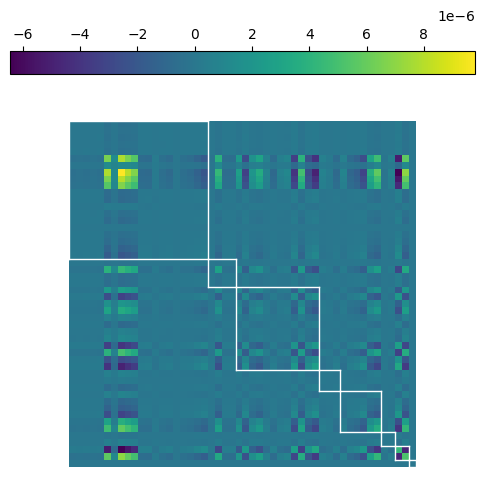
\includegraphics[width=0.43\linewidth]{kfac_pinns_exp/exp04_gramian_contributions/fig/gram_full.png}

  \begin{tabular}{ccc}
    (\textcolor{blue}{forward}, \textcolor{red}{forward})
    &
      (\textcolor{blue}{forward}, \textcolor{red}{gradient})
    &
      (\textcolor{blue}{forward}, \textcolor{red}{Hessian})
    \\
    
\includegraphics[width=0.22\linewidth]{kfac_pinns_exp/exp04_gramian_contributions/fig/gram_output_output.png}
    &
      
\includegraphics[width=0.22\linewidth]{kfac_pinns_exp/exp04_gramian_contributions/fig/gram_output_grad_input.png}
    &
      
\includegraphics[width=0.22\linewidth]{kfac_pinns_exp/exp04_gramian_contributions/fig/gram_output_hess_input.png}
    \\
    (\textcolor{blue}{gradient}, \textcolor{red}{forward})
    &
      (\textcolor{blue}{gradient}, \textcolor{red}{gradient})
    &
      (\textcolor{blue}{gradient}, \textcolor{red}{Hessian})
    \\
    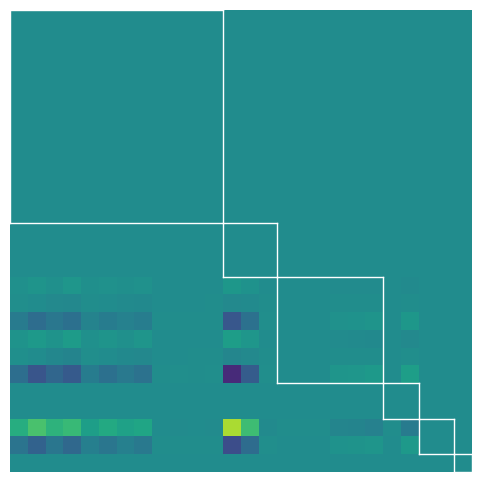
\includegraphics[width=0.22\linewidth]{kfac_pinns_exp/exp04_gramian_contributions/fig/gram_grad_input_output.png}
    &
      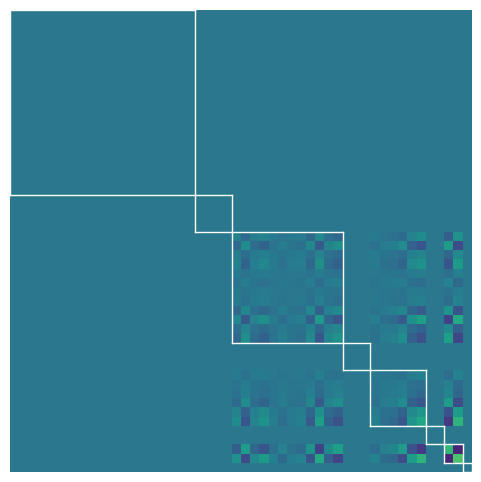
\includegraphics[width=0.22\linewidth]{kfac_pinns_exp/exp04_gramian_contributions/fig/gram_grad_input_grad_input.png}
    &
      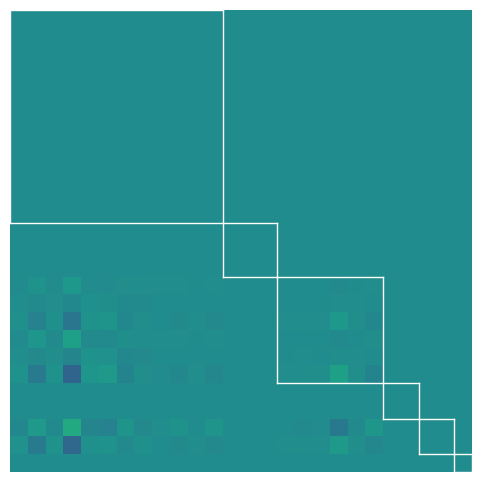
\includegraphics[width=0.22\linewidth]{kfac_pinns_exp/exp04_gramian_contributions/fig/gram_grad_input_hess_input.png}
    \\
    (\textcolor{blue}{Hessian}, \textcolor{red}{forward})
    &
      (\textcolor{blue}{Hessian}, \textcolor{red}{gradient})
    &
      (\textcolor{blue}{Hessian}, \textcolor{red}{Hessian})
    \\
    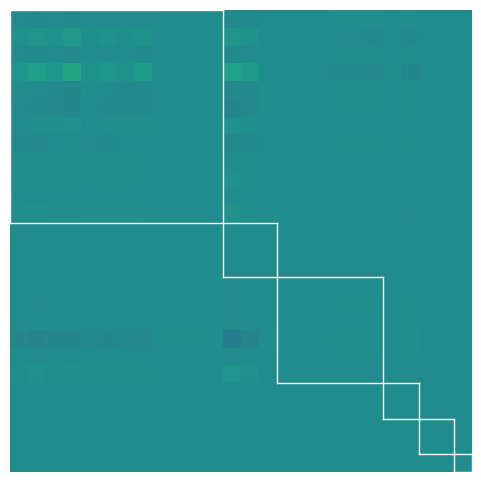
\includegraphics[width=0.22\linewidth]{kfac_pinns_exp/exp04_gramian_contributions/fig/gram_hess_input_output.png}
    &
      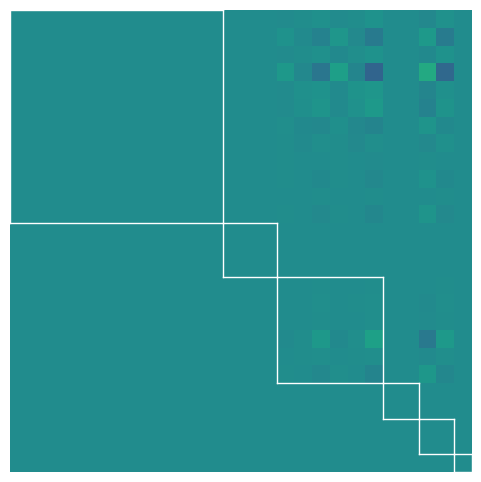
\includegraphics[width=0.22\linewidth]{kfac_pinns_exp/exp04_gramian_contributions/fig/gram_hess_input_grad_input.png}
    &
      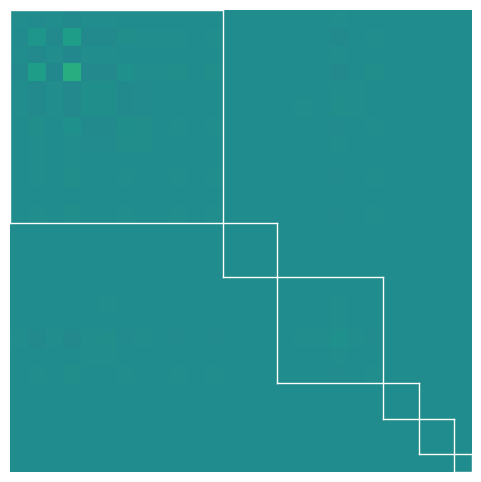
\includegraphics[width=0.22\linewidth]{kfac_pinns_exp/exp04_gramian_contributions/fig/gram_hess_input_hess_input.png}
  \end{tabular}
  \caption{Contributions $\mG_{\Omega,\textcolor{blue}{\bullet}, \textcolor{red}{\bullet}}$ to the Laplacian's Gramian $\mG_{\Omega}$ from different children in the computation graph on a synthetic toy problem.
    We use a $4 \to 3 \to 2 \to 1$ sigmoid-activated MLP and 10 randomly generated inputs. The contributions are highlighted as in \Cref{eq:fisher}.}\label{fig:gramian-contribution-children}
\end{figure}
%%% Local Variables:
%%% mode: latex
%%% TeX-master: "../main"
%%% End:


\paragraph{Computing $\jac_{\mW^{(i)}}\bullet$}
Let us first compute the Jacobians $\jac_{\mW^{(i)}}\bullet$ in \Cref{eq:laplacian-gradient}.
The Jacobian of the linear layer's forward pass is
\begin{subequations}\label{eq:fisher-jacobians}
  \begin{align}
    \jac_{\mW}\left( \mW \vx \right) = \vx^{\top} \otimes \mI\,.
  \end{align}
  The Jacobian from the gradient backpropagation is
  \begin{align}
    \jac_{\mW}\left( \mW^{\top} \vx \right) = \mI \otimes \vx^{\top}\,,
  \end{align}
  and the Jacobian from the Hessian backpropagation is
  \begin{align}\label{subeq:fisher-jacobians-hbp}
    \jac_{\mW}\left( \mW^{\top} \mX \mW \right)
    =
    \mI \otimes \mW^{\top}\mX
    +
    \mK \left(
    \mI
    \otimes
    \mW^{\top}\mX^{\top}
    \right)\,,
  \end{align}
\end{subequations}
where $\mK \in \sR^{\dim(\mZ) \times \dim(\mZ)}$ (denoting $\mZ := \mW^{\top}\mX \mW$) is a permutation matrix that, when multiplied onto a vector whose basis corresponds to that of the flattened output $\mZ$, modifies the order from first-varies-fastest to last-varies-fastest, i.e.
\begin{equation*}
  \mK \flatten(\mZ) = \flatten(\mZ^{\top})\,.
\end{equation*}
Re-introducing the layer indices, the expressions in \Cref{eq:spatialDerivatives} become
\begin{align}
  \begin{split}
    \jac_{\mW^{(i)}}\vz^{(i)}
    &=
      {\vz^{(i-1)}}^\top\otimes \mI
    \\
    \jac_{\mW^{(i)}}\grad{\vz^{(i-1)}}u\,,
    &=
      \mI\otimes
      \grad{\vz^{(i)}}u
    \\
    \jac_{\mW^{(i)}}\gradsquared{\vz^{(i-1)}}u\,,
    &=
      \mI \otimes
      \left[
      {\mW^{(i)}}^{\top}
      \left(
      \gradsquared{\vz^{(i)}}u
      \right)
      \right]
      +
      \mK
      \left(
      \mI \otimes
      \left[
      {\mW^{(i)}}^{\top}
      \left(
      \gradsquared{\vz^{(i)}}u
      \right)^{\top}
      \right]
      \right)\,.
  \end{split}
\end{align}
We will now use symmetries in the objects used during Hessian backpropagation to simplify this further.
At a first glance, it looks like the Gramian consists of 16 terms, as there are 4 summands from the Jacobians in \Cref{eq:fisher-jacobians}.
However, we can simplify into 9 terms:

First, $\gradsquared{\vz^{(i)}}u$ is symmetric, that is
\begin{align*}
  \jac_{\mW^{(i)}}\left( {\mW^{(i)}}^{\top} \left( \gradsquared{\vz^{(i)}}u  \right)\mW^{(i)} \right)
  &=
    \mI \otimes
    \left[
    {\mW^{(i)}}^{\top} \left( \gradsquared{\vz^{(i)}}u  \right)
    \right]
    +
    \mK
    \left(
    \mI \otimes
    \left[
    {\mW^{(i)}}^{\top}
    \left(
    \gradsquared{\vz^{(i)}}u
    \right)
    \right]
    \right)\,,
    \shortintertext{and the transposed Jacobian is}
  &\mI \otimes
    \left[
    \left( \gradsquared{\vz^{(i)}}u  \right) \mW^{(i)}
    \right]
    +
    \left(
    \mI \otimes
    \left[
    \left(
    \gradsquared{\vz^{(i)}}u
    \right)
    \mW^{(i)}
    \right]
    \right)
    \mK^{\top}\,.
\end{align*}
Second, we multiply the transpose Jacobian onto $\grad{\gradsquared{\vz^{(i-1)}}u}\Delta u$, which inherits symmetry from the Hessian, $[\grad{\gradsquared{\vz^{(i-1)}}u}\Delta u]_{j,k} = [\grad{\gradsquared{\vz^{(i-1)}}u}\Delta u]_{k,j}$.
Due to this symmetry, the action of $\mK$ (or $\mK^{\top}$) does not alter it,
\begin{align*}
  \mK^{\top}\left( \grad{\gradsquared{\vz^{(i-1)}}u}\Delta u \right) = \grad{\gradsquared{\vz^{(i-1)}}u}\Delta u\,.
\end{align*}
In other words, it does not matter how we flatten (first- or last-varies-fastest).
This simplifies the VJP (last line in \Cref{eq:fisher}) to
\begin{align*}
  \left(
  \mI \otimes
  \left[
  \left( \gradsquared{\vz^{(i)}}u  \right) \mW^{(i)}
  \right]
  \right)
  \grad{\gradsquared{\vz^{(i-1)}}u}\Delta u
  +
  \left(
  \mI \otimes
  \left[
  \left(
  \gradsquared{\vz^{(i)}}u
  \right)
  \mW^{(i)}
  \right]
  \right)
  \mK^{\top}
  \grad{\gradsquared{\vz^{(i-1)}}u}\Delta u
  \\
  =
  2 \left(
  \mI \otimes
  \left[
  \left( \gradsquared{\vz^{(i)}}u  \right) \mW^{(i)}
  \right]
  \right)
  \grad{\gradsquared{\vz^{(i-1)}}u}\Delta u
  \,.
\end{align*}
We can now write down the simplified Jacobian from \Cref{eq:laplacian-gradient}, whose self-outer product forms the Gramian block for a linear layer's weight matrix,
\begin{align}\label{eq:weight-jacobian-simplified}
  \begin{split}
    \jac_{\mW^{(i)}} \Delta u
    &=
      \underbrace{
      \left(
      {\vz^{(i-1)}}^\top\otimes \mI
      \right)^{\top}
      \grad{\vz^{(i)}}\Delta u
      }_{(1)}
    \\
    &\phantom{=}+
      \underbrace{
      \left(
      \mI \otimes \grad{\vz^{(i)}}u
      \right)^{\top}
      \grad{\grad{\vz^{(i-1)}}u}\Delta u
      }_{(2)}
    \\
    &\phantom{=}+
      \underbrace{
      2
      \left(
      \mI \otimes
      \left[
      \left( \gradsquared{\vz^{(i)}}u \right) \mW^{(i)}
      \right]
      \right)
      \grad{\gradsquared{\vz^{(i-1)}}u}\Delta u
      }_{(3)}
      \,,
  \end{split}
\end{align}
where (1) is the contribution from the forward pass, (2) is the contribution from the gradient backpropagation, and (3) is the contribution from the Hessian backpropagation. The Jacobians from \Cref{eq:fisher-jacobians} allow to express the Gramian in terms of Kronecker-structured expressions consisting of 9 terms in total. \Cref{fig:gramian-contribution-children} shows the 6 contributions from different children pairs.

\paragraph{Conclusion} One problem of computing the Laplacian and its Jacobian with backpropagation according to \Cref{eq:weight-jacobian-simplified} is that if we write out the Gramian's block $\mG_{\Omega}^{(i)} = \jac_{\mW^{(i)}} \Delta u (\jac_{\mW^{(i)}} \Delta u)^{\top}$, we obtain 9 terms of different structure.
Defining a single Kronecker product approximation would involve introducing new approximations on top of those employed by \citet{eschenhagen2023kroneckerfactored}.
Therefore, the forward Laplacian, or Taylor-mode, perspective we choose in the main text is advantageous as it allows to define KFAC without introducing new approximations.

\paragraph{Computing $\grad{\textcolor{blue}{\bullet}}\Delta u$}
The terms $\grad{\textcolor{blue}{\bullet}}\Delta u$ are automatically computed when computing the gradient of the loss via backdrop.

%%% Local Variables:
%%% mode: latex
%%% TeX-master: "../main"
%%% End:



%%% Local Variables:
%%% mode: latex
%%% TeX-master: "../main"
%%% End:
